% E7: the production book translation on raw-API ranks, one node to many.
% Every number is a macro from paper/e7_results.tex, generated by
% experiments/e7_rawapi_book/analyze.py from the sealed runs under runs/e7-rawapi-*.

\subsection{E7: the production translation, from one machine to eight}
\label{sec:eval-e7}

E3 wrote the protocol for this task and could not staff it. Its executors were
agent-host sessions; the host capped concurrent sessions at ten; and every run
above $p=16$ spent its wall time waiting for an executor to exist
(the record is on the branch that wrote it). E7 keeps E3's design---the same collectives, for the same
reasons---and changes what a rank \emph{is}. A rank is an operating-system
process. Its executor is a chat-completions call with a bounded tool loop. It is
started by \code{ampirun}, the process manager the standard leaves unspecified,
on one machine or across several. Executor supply stops being the experiment's
limiting resource, so for the first time the population can be scaled against a
fixed workload: the same 2013 Russian biography, \eSevenScales\ scales from
$p=16$ on one machine to $p=\eSevenLargest$ over eight.

\paragraph{What changed, and why.}
Four things distinguish E7 from E3, and each is a protocol mechanism rather than a
prompt.

\emph{The unit is the paragraph.} A page-cut book has 95 prose pages; a
paragraph-cut one has 1232, so $p$ can reach 256 with two to five paragraphs a
rank. Segments stay contiguous and character-balanced, and the seam exchange
keeps its meaning.

\emph{Arbitration is agent-evaluated and parallel.} E3's root settled lifted
conflicts with the runtime's default rule, which chooses a candidate and
exercises no judgement. Here the root asks a model---but not alone. After the
\code{allreduce} every rank holds the same conflict set, so rank $r$ arbitrates
batch $r$ of it, the rulings are gathered to the root, and the root commits them
with \code{op\_arbitrate} exactly once. The serial step that would otherwise
grow with the population is spread over it; what remains serial is one
\code{gather} and one commit.

\emph{Results are checkpointed and collectives replay.} Every agent result is
written to a window before the rank proceeds. A rank whose process dies is
restarted by \code{ampirun} through the runtime's \code{respawn}, receives a new
epoch, and re-enters the same program: each collective it already joined returns
its stored result (the completion is traced \code{replayed}, with its wait
measured from re-entry), each task it already finished is read back, and it
resumes at the first thing its predecessor did not finish. With
\code{--die-fraction} a chosen fraction of ranks exits mid-phase, so the cost of
the lifecycle failure every multi-agent postmortem reports becomes a measured
quantity.

\emph{Shared state under a lock.} A translator who settles a term the glossary
did not cover records it in a per-chapter ledger under an exclusive, leased,
fenced window lock, first writer wins. The merge needs a judgement
\code{accumulate} cannot make---a term already present with a different
rendering is a clash to record, not a value to overwrite---so this is the one
place the harness locks, and the lock's contention is in the trace.

\paragraph{The executor.}
A raw endpoint has no body. The executor (\code{ampi/model.py}) gives it the
smallest one that suffices: an encyclopaedia search, an article, a page fetch,
called through the provider's function-calling schema in a loop bounded both by
steps and by cumulative prompt tokens. Contract violations are repaired in the
same conversation rather than by a fresh attempt. Every call's exact prompt and
completion tokens, tool calls and cost land in the trace as \code{task.*}
events, which the analysis reads as it reads the broker's claim/submit pair.
Two things the executor taught us are recorded as defects fixed. A tool loop
whose tools are silently withdrawn produces empty replies; withdrawing them in
the model's own turn does not. And a rate limit is not a failure of a task: the
first production attempt lost six ranks to a twenty-requests-a-minute cap because
429s were retried like transport faults, six times and then never. A rank waiting
on a rate limit is a rank blocked, exactly like one blocked in a collective, and
the wait is now bounded by patience rather than by a count.

\paragraph{The population is heterogeneous by necessity.}
The provider caps every capable model at twenty requests a minute \emph{per
model} for the account these runs used. A population of sixty-four ranks on one
model would queue on the cap rather than translate. So rank $r$ runs model
$r \bmod 8$ of a pool of eight, at every scale, which multiplies the aggregate
limit by eight and makes the executors heterogeneous in a way the protocol never
asks about. A segment's model is a function of its rank alone, the mix is the
same across the series, and the trace records the model behind every task, so
per-model latency and cost are a by-product of the run rather than an extra
experiment.

\paragraph{Across machines.}
The single-node runs use the SQLite device and sixteen to sixty-four processes
on a four-core sandbox; the processes are network-bound and the core count does
not matter. The multi-node runs use \code{gitd}, the git device behind a per-node
daemon (\S\ref{sec:impl}). E5 measured the git device at one push per mutation:
thirty-two ranks on thirty-two machines made 1131 pushes and suffered 13415
rejections in forty-two minutes for four collectives. The daemon owns the working
tree on each machine and group-commits every mutation its ranks issue within a
window---the intra-node aggregation every production MPI performs before it
touches the interconnect---so the pushes on the wire are bounded by the machine's
rate of bursts, not its ranks' rate of operations. The guarantee each rank sees is
unchanged. With stub executors, eight ranks over two machines and a hosted remote
made 1371 operations in 441 pushes; the median collective's slowest participant
waited a minute, against a second on one machine. That minute is the price of
sharing nothing but a git remote, and the question the multi-node runs answer is
whether it matters against an executor whose one step costs minutes.

\paragraph{Method.}
Every run cuts the same book by the same rule, uses the same prompts, the same
research cap (48 terms) and budget (3 per rank), the same model pool, and the
same policies (quorum 1, barrier policy \emph{proceed}, one restart per rank).
What changes with $p$ is the segment size and the number of segments: strong
scaling. The launch plan names every rank requested before any runs; each node's
launch record carries the machine's kernel boot id; each rank's report carries
its epoch and the model it ran on; and the trace carries everything else. The
source is in copyright and never leaves the untracked working directory; the
repository carries the evidence, the population's glossary, its research
findings with their sources, and its amendment ledger.

\paragraph{Results.}
%% RESULTS: filled in from the sealed runs; see the table and figures below.
% Results prose for the E7 section.  Numbers come from the macros in
% e7_results.tex (generated); the qualitative claims are read off the sealed runs
% under runs/e7-rawapi-* and runs/e7-series.

\emph{The population finishes, and the protocol never wedges.}  Every run in
Table~\ref{tab:e7} closed all of its collectives and assembled a book.  At
$p=16$ the sixteen processes rendered \eSevenCoverageSixteen\% of the 1232
paragraphs in \eSevenWallSixteen\ minutes for \$\eSevenCostSixteen; at $p=64$,
\eSevenCoverageSixtyfour\% in \eSevenWallSixtyfour\ minutes for
\$\eSevenCostSixtyfour.  The coverage that is missing is not the protocol's:
it is the segments of ranks whose model degenerated (below), which the runtime
dropped from their collectives after the restart budget was spent so that the
rest of the population could close.

\emph{More ranks bought little wall time, and the trace says why.}  Wall time
fell from \eSevenWallSixteen\ to \eSevenWallThirtytwo\ to
\eSevenWallSixtyfour\ minutes as $p$ quadrupled, while executor work stayed near
\eSevenWorkHSixteen--\eSevenWorkHSixtyfour\ rank-hours and blocked time grew
from \eSevenBlockedHSixteen\ to \eSevenBlockedHSixtyfour\ rank-hours: the
coordination share rose from \eSevenCoordShareSixteen\% to
\eSevenCoordShareSixtyfour\%, and parallel efficiency fell from
\eSevenEfficiencySixteen\% to \eSevenEfficiencySixtyfour\%.  This is not
protocol overhead.  On one machine the median collective released its slowest
participant within a second.  It is Amdahl with a heterogeneous denominator:
the run ends when its last rank ends, and the last rank is decided by which
model it drew.  Across the three runs the median translation chunk took
28~s on the fastest model in the pool and 119~s on the slowest, a 4.3$\times$
spread (Figure~\ref{fig:e7models}); the longest single wait in every run was a
seam exchange or the final spend reduction blocked on one rank whose model
was slow, or had failed and been restarted.  With a fixed book, adding ranks
shortens every rank's segment but does not shorten the slowest model's
proportion of it.

\emph{What the collectives did.}  The census lifted \eSevenConflictsSixteen,
\eSevenConflictsThirtytwo\ and \eSevenConflictsSixtyfour\ conflicts at the
three scales---renderings on which ranks reading different parts of the book
disagreed---and every one was arbitrated exactly once by a model, in parallel
batches, before the research agenda was built from them.  The 48 researched
terms cite \eSevenSourcesSixteen\ sources at $p=16$ and were each researched
by exactly one rank at every scale: the compare-and-swap claim on the research
window is what turned 64 potential investigations of ``Дом Зингера'' into one.
The glossary that bound the translation grew from \eSevenGlossarySixteen\ to
\eSevenGlossarySixtyfour\ terms with $p$, because more ranks survey more
finely; the amendment ledger, written under the per-chapter lock, recorded
\eSevenAmendmentsSixteen, \eSevenAmendmentsThirtytwo\ and
\eSevenAmendmentsSixtyfour\ terms translators settled themselves, with
\eSevenClashesSixteen, \eSevenClashesThirtytwo\ and \eSevenClashesSixtyfour\
clashes---two ranks settling the same term differently in the same chapter---
which is exactly the number the glossary phase had failed to prevent, and which
the ledger exists to make visible.

\emph{Failures were contained, and they were instructive.}  \eSevenRestartsSixteen,
\eSevenRestartsThirtytwo\ and \eSevenRestartsSixtyfour\ ranks were restarted by
\code{ampirun} at the three scales; each successor took a new epoch, re-entered
its closed collectives (\eSevenReplaysNote), read back its finished tasks, and
resumed.  Most restarts at $p=64$ had one cause, a race in the harness that
delivered broadcast bodies to a file shared between ranks, found and fixed
while the run was in progress; a rank restarted after the fix ran the fixed
code, which is a property of process ranks that session ranks do not have.
The failures that cost coverage had a different cause: one model in the pool
degenerated into thousands of blank lines mid-object on the same paragraphs
three times running, and in-conversation repair only reproduced the
degeneration.  A homogeneous population has no answer to that; a heterogeneous
one does, and the executor now falls back to a second model from a fresh
conversation when the first exhausts its attempts.  The multi-node runs carry
that fix; the single-node runs above do not, and the difference is reported
rather than hidden.

\emph{Rate limits are a shared resource, and the trace measures them.}  Every
capable model on the account was capped at twenty requests a minute, per
model.  The eight-model pool is what let sixty-four ranks proceed at all; the
first attempt on one model lost six ranks to the cap before rate limits were
made a wait rather than a failure.  The executor now records the time it spent
rate-limited, so at $p=256$ the cost of the cap is a number in the trace
rather than an inference from wall time.

\emph{Across machines.}  \eSevenMultiNodeNote


\begin{table}[t]
\centering\small
\begin{tabular}{rrrrrrrrr}
\toprule
$p$ & nodes & wall (min) & tasks & restarts & coord.\ share & efficiency & spend (\$) & coverage \\
\midrule
\eSevenTableRows
\bottomrule
\end{tabular}
\caption{E7 across scales. Coordination share is blocked rank-seconds over all
rank-seconds; efficiency is achieved parallelism over $p$; coverage is the
fraction of the 1232 paragraphs rendered into all three languages.}
\label{tab:e7}
\end{table}

\begin{figure}[t]
\centering
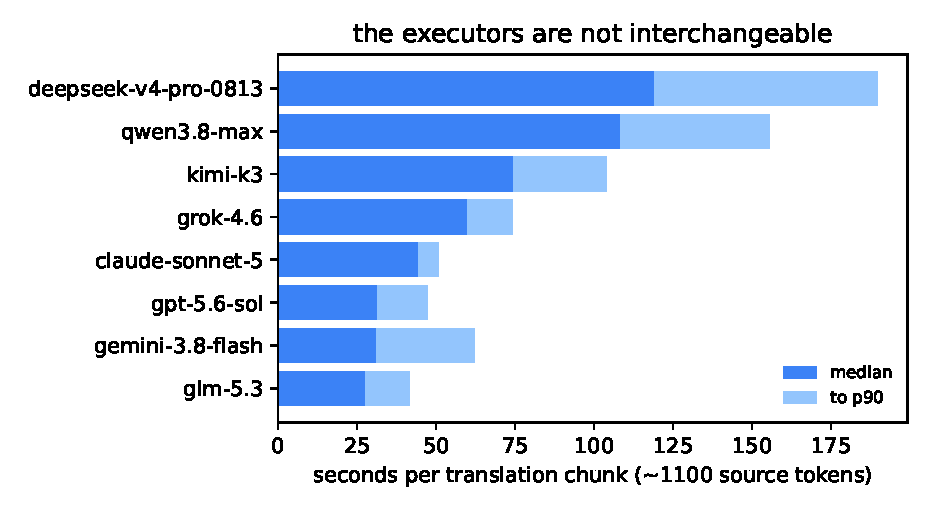
\includegraphics[width=0.7\linewidth]{../runs/e7-series/latency_by_model.pdf}
\caption{Seconds per translation chunk (about 1100 source tokens into three
languages) by model, pooled over the single-node runs: median, and median to
90th percentile.  Rank $r$ ran model $r \bmod 8$; the run ends when the slowest
of them does.}
\label{fig:e7models}
\end{figure}

\begin{figure}[t]
\centering
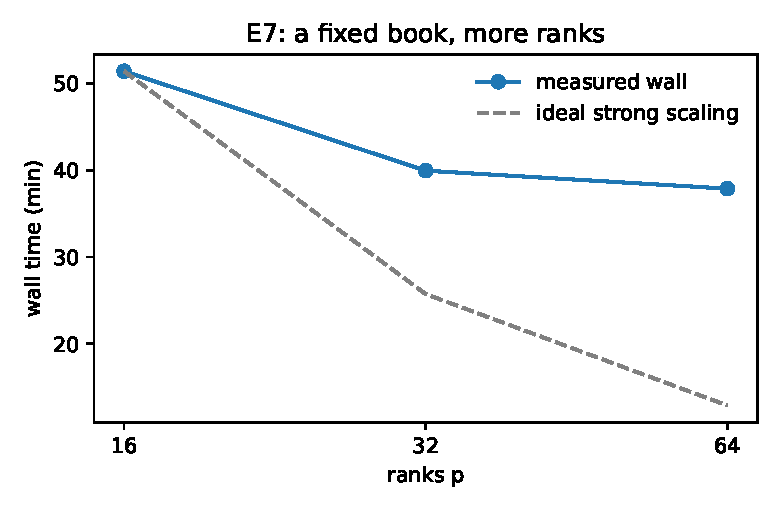
\includegraphics[width=0.48\linewidth]{../runs/e7-series/wall_vs_p.pdf}\hfill
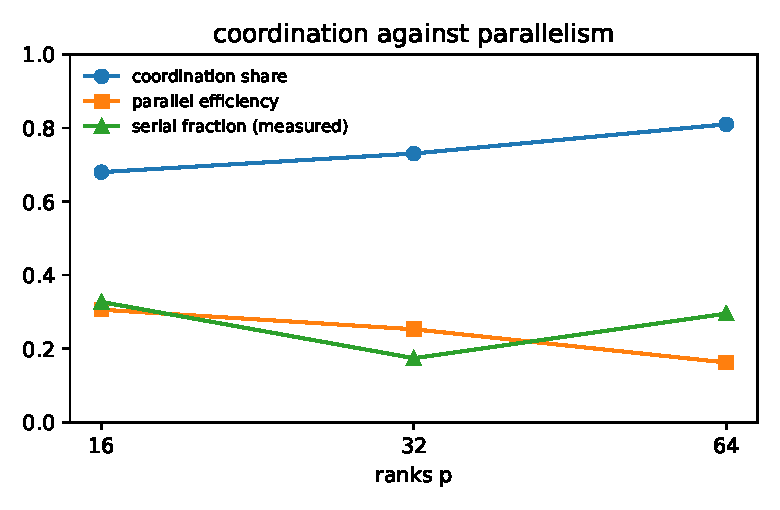
\includegraphics[width=0.48\linewidth]{../runs/e7-series/efficiency_vs_p.pdf}
\caption{Left: wall time against $p$ for a fixed book, with ideal strong scaling.
Right: coordination share, parallel efficiency, and the measured serial fraction.}
\label{fig:e7scaling}
\end{figure}
